\documentclass[10pt,a4paper]{article}

\usepackage{amsmath}
\usepackage{amsfonts}
\usepackage{amssymb}
\usepackage{graphicx} 
\usepackage[german]{babel}
\usepackage[utf8]{inputenc}
\usepackage{listings} %For code

\begin{document}

%Titelseite
\begin{titlepage}

\begin{center}
\vspace*{1.3cm}
{\Huge Dependable Systems\\(VU 182.712)\\}
\vspace{1.7cm}
{\LARGE Praktisches Ubungsbeispiel SS2015:\\``Zuverl�assigkeitsmodellierung mit \textit{sharpe}''\\}
\vspace{1.7cm}


{\hspace{1cm} Datum der Labor�bung: 18.06.2015}


\begin{table}[h!]
\centering
\begin{tabular}{|p{3.5cm}|p{6.5cm}|}
\hline \textbf{Matr. Nr.} & \textbf{Name} \\
\hline
1228774 &  Schieber Constantin \\
\hline
&  Pacheiner Peter \\
\hline
1226314 & Hofer David \\
\hline
\end{tabular}
\end{table}

\end{center}
\vspace{1.0cm}

\end{titlepage}
\setcounter{page}{2}






\newpage
\section{Abstract}
Ein Computernetzwerk soll durch Markovketten modelliert werden um es auf Fehlersicherheit zu überprüfen.
\\ 
Konkret soll die Mean Time to Failure (MTTF) und die Verfügbarkeit zwischen 2 Systemen evaluiert und verglichen werden. Eines ohne Redundanz und eines mit.
Zusätzlich soll ein Vergleich zwischen den Kosten für die beiden Systeme durchgeführt werden.

\section{Executive Summary}
Es wurden 4 verschiedene Systeme mit Markovketten modelliert:
\begin{itemize}
	\item Das einfache Modell
	\item Das redundante Modell mit absorbierenden Zustand
	\item Das einfache Modell mit Reparaturkanten
	\item Das redundante Modell mit Reparaturkanten
\end{itemize}
In Punkt \ref{subsec:mttf_res} wird die MTTF anhand der ersten 2 Modelle simuliert und das Ergebnis ausgewertet. In Punkt \ref{subsec:avail_res} wird anhand der letzten 2 Modelle die Availability des Systems simuliert und das Ergebnis ausgewertet. \\
Unter Punkt \ref{sec:cost} werden die Kostenunterschiede zwischen redundanten und einfachen Systemen diskutiert und eine Grenze, ab der sich ein redundantes System für unser Problem auszahlt, berechnet.
\newpage
\section{Aufgabenstellung}
Für beide Systeme gelten die folgenden Fehlerraten ($\lambda$) und Reparaturraten ($\mu$).
\begin{itemize}
	\item $\lambda_R=10^{-4}/Std.$ für Rechner
	\item $\lambda_N=2*10^{-5}/Std.$ für Switches
	\item  $\mu=10^{-2}/Std. $ für Beide
	
Um funktionsfähig zu sein benötigt das Netzwerk mindestens einen Switch und drei Rechner.
\end{itemize}
\section{Mean Time to Failure} 
\label{sec:mttf}
\subsection{Einfaches System}
Das Computernetzwerk besteht aus drei über einen Switch verbunden Rechnern.
\\
Um die MTTF zu evaluieren reicht es das System durch 2 Zustände zu modellieren. \\
Einer stellt den funktionierenden Zustand (0) dar, der andere den Fehlerzustand (1).
Die Wahrscheinlichkeit für einen Übergang in den Fehlerzustand setzt sich dann aus $3*\lambda_R + \lambda_N$ zusammen. Diese Vereinfachung kann vorgenommen werden da jeder Ausfall, egal welcher Art, in einen Fehlerzustand führt. 
Die Reparaturrate muss nicht berücksichtigt werden da wir uns im Moment ausschließlich für die MTTF interessieren.
\\
Das System kann sowohl graphisch als auch in Textform beschrieben werden:
\begin{figure}[ht!]
\centering
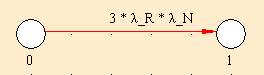
\includegraphics[width=90mm]{MTTM_EinfachesModell.png}
\caption{Einfaches System in \textit{sharpe} modelliert \label{mmtm_einfach}}
\end{figure}

\lstinputlisting{MTTF_Einfach_Modell.txt}
\subsection{Redundantes System}
Das redundante Computernetzwerk besteht aus 4 Rechnern und 2 Switches was die Ausfallwahrscheinlichkeit gegenüber dem einfachen System deutlich verringern sollte.\\
Statt 2 Knoten werden nun 5 Knoten benötigt um alle Übergänge korrekt abzubilden.\\
Das System ist in den Knoten 0,1,2,3 funktionsfähig, Knoten 4 ist der Fehlerzustand (siehe Grafik \ref{mmtm_redundant}).
\begin{figure}[ht!]
\centering
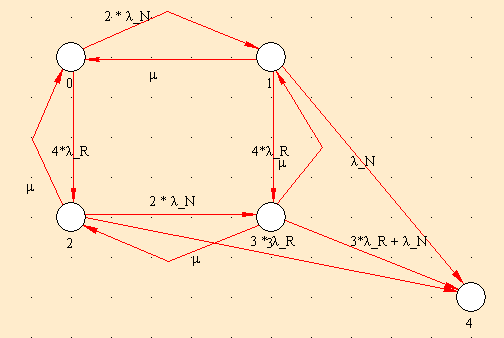
\includegraphics[width=90mm]{MTTM_ReduntantesModell.png}
\caption{Redundantes System in \textit{sharpe} modelliert \label{mmtm_redundant}}
\end{figure}
\lstinputlisting{MTTF_Redundant_Modell.txt}
\newpage
\subsection{Vergleich der beiden Systeme}
\label{subsec:mttf_res}
Um die beiden Systeme vergleichen zu können muss nun auch die Simulation derselbigen durchgeführt werden. Dies geschieht durch folgende Befehlsseqünz in \textit{sharpe}:
\lstinputlisting{MTTF.txt}

\textbf{Daraus resultieren die folgenden Ergebnisse:} 
\lstinputlisting{MTTF_RESULTS.txt}
Das bedeutet dass das einfache Modell nach ca. 3125 Stunden ausfällt und das Redundante erst nach 8854 Stunden. Man sieht dass sich durch das hinzufügen der Redundanz der Zeitraum bis zum Ausfall deutlich erhöht.
Zusätzlich zu den beiden genannten Modellen wurde aus Interesse ein drittes Modell getestet welches
zwar redundant ist aber absolut keine Reparaturkanten besitzt. Wie man sehen kann ist bei diesem System eine Zeit von 5767 Stunden bis zum ersten Ausfall angegeben. 
Das ergibt 'nur' 2632 Stunden mehr als bei einem einfachen System. Man kann also deutlich sehen dass ein redundantes System zwar die Ausfallsicherheit erhöht, ohne ausreichend schnelle Reparatur aber
schnell das selbe Schicksal wie ein einfaches (und damit billigeres) System erleidet.
\\
Um die Unterschiede zu verdeutlichen wurde ein Diagramm (Abb. \ref{fail_plot}) erstellt. In diesem kann man gut erkennen dass der Unterschied zwischen dem Einfachen und dem redundanten System ohne Reparaturkanten vernachlässigbar klein ist.

Mit \textit{sharpe} ist es möglich sich die "Cumulative Distribution Function" zu berechnen.
Mit dieser Funktion lässt sich bestimmen welchen Wert eine Zufallsvariable $x$ maximal annimmt (zwischen 0 und 1). \\
Der Aufruf inklusive Ausgabe der Werte sieht dann so aus:
\lstinputlisting{MTTF_CDF_SAMPLE.txt}
Diese Funktion wurde auf die drei Systeme angewandt und sieht als Plot folgendermaßen aus:

\begin{figure}[ht!]
\centering
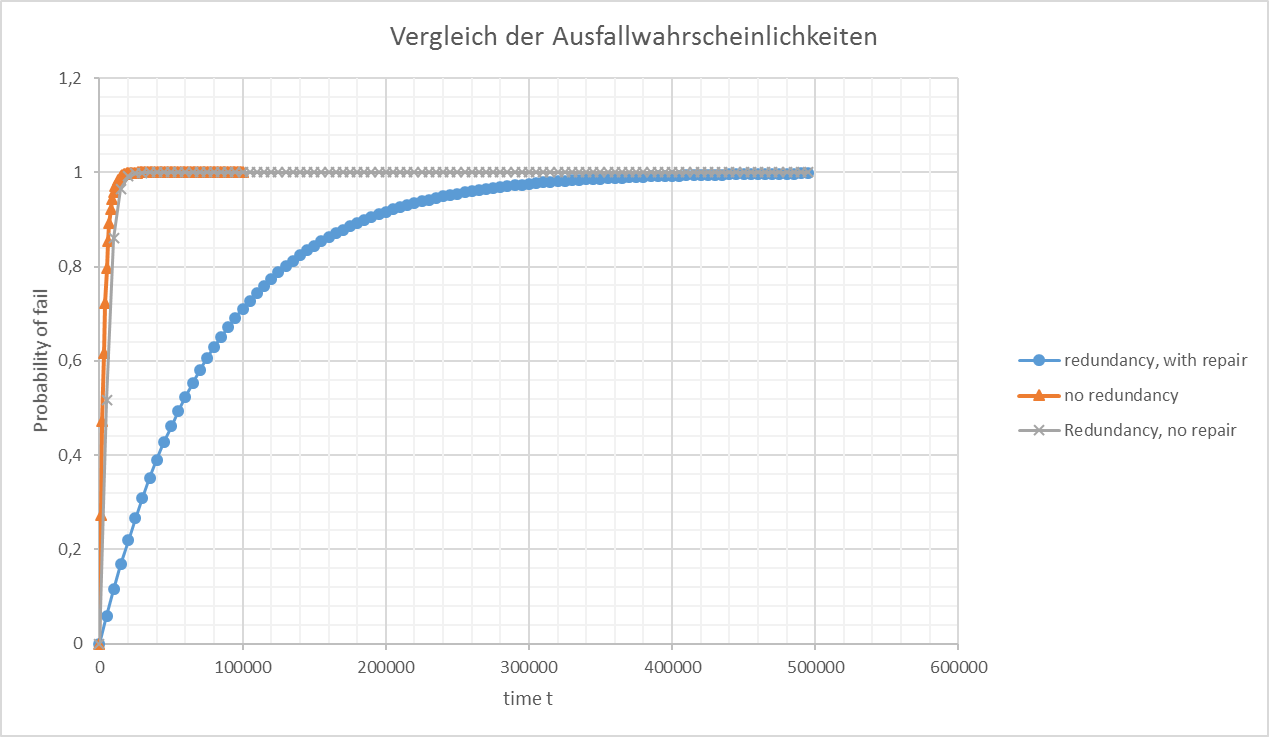
\includegraphics[width=140mm]{Ausfallwahrscheinlichkeit_Plot.png}
\caption{Unterschiedliche Strategien für Systeme \label{fail_plot}}
\end{figure}

\section{Availability}
\label{sec:avail}
Im Gegensatz zur MTTF ist bei der Availability die Reparaturrate nun auch vom Fehlzustand aus zu berücksichtigen.
\subsection{Einfaches System}
Für das einfache System wird einfach eine neue Kante die zurück in den funktionierenden Zustand führt hinzugefügt.
\begin{figure}[ht!]
\centering
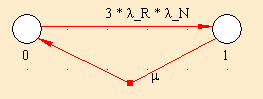
\includegraphics[width=90mm]{AVAILABILITY_Einfach.png}
\caption{Einfaches System mit neür Kante in \textit{sharpe} modelliert \label{avail_einfach}}
\end{figure}
\lstinputlisting{AVAILABILITY_Einfach.txt}
\newpage
\subsection{Redundantes System}
Im redundanten System reicht nun ein Fehlerzustand nicht mehr aus da wir aus diesem auch wieder zurück kehren können. Um sich den Zustand des restlichen Systems zu "merken" bzw.. um deterministisch agieren zu können werden 3 neue Knoten eingeführt, die jeweils als Fehlzustände fungieren und über eine Kante mit dem letzten funktionierenden Zustand verbunden sind. 
\begin{figure}[ht!]
\centering
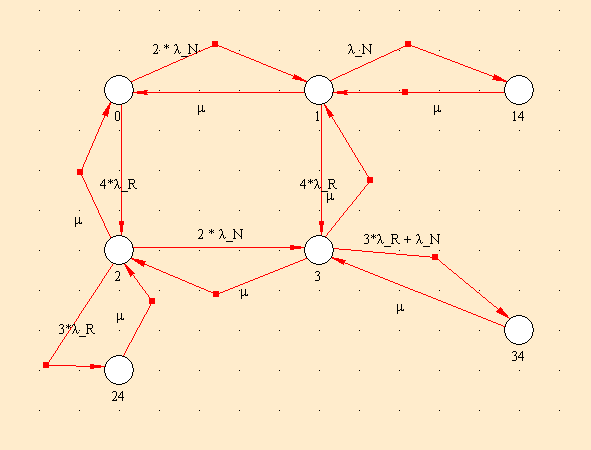
\includegraphics[width=90mm]{AVAILABILITY_RED.png}
\caption{Redundantes System in \textit{sharpe} modelliert \label{avail_einfach}}
\end{figure}
\lstinputlisting{AVAILABILITY_RED.txt}
\newpage
\subsection{Vergleich der beiden Systeme}
\label{subsec:avail_res}
Der Vergleich der beiden Systeme wird mit dem Befehl \textit{prob(SYS, NODE)} ausgeführt. Dieser errechnet die Zustandswahrscheinlichkeit für eine bestimmte \textit{NODE} im angegebenen System.\\
Im einfachen System reicht es die Wahrscheinlichkeit berechnen zu lassen mit der sich das System im gültigen Zustand befindet. \\
Im redundanten Fall ist es einfacher die Wahrscheinlichkeit der Fehlzustände berechnen zu lassen, diese zu addieren und von 100\% abzuziehen.

Der Aufbau der Befehlsabfolge sieht so aus:
\lstinputlisting{AVAILABILITY.txt}
\newpage
Und das Ergebnis dann folgendermaßen:
\lstinputlisting{AVAILABILITY_RESULTS.txt}
Wie man sieht beträgt die Wahrscheinlichkeit dafür dass sich das einfache System in einem gültigen Zustand befindet $96.899\%$. \\
Die Wahrscheinlichkeit in einem redundanten System beträgt $99.87\%$.
\section{Kosten}
\label{sec:cost}
Abschlie{\ss}end soll noch berechnet werden, ab welchem Verh\"altnis von
Ausfallkosten zu Normalbetriebskosten des Systems, die fehlertolerant
erweiterte Systemvariante zu bevorzugen ist. Laut Angabe ist der Normalbetrieb der erweiterten Variante 2.5 mal
so teuer wie der Normalbetrieb der einfachen Variante. W\"ahrend sich ein System
im ausgefallenen Zustand befindet, verursacht es laufende
Ausfallkosten, die sich auf ein Vielfaches der Betriebskosten der einfachen Variante belaufen.


\bigskip

In den weiteren Berechnung werden die folgenden Bezeichnungen verwendet:


\bigskip

 $K_{\mathit{Normalbetrieb}}$: Kosten f\"ur den Normalbetrieb des
einfachen Systems

 $K_{\mathit{Ausfall}}$ : laufende Ausfallkosten, im Fall dass sich das
System im Zustand \ {\quotedblbase}Ausgefallen{\textquotedblleft}
befindet.

 $K_{\mathit{GS}}$ : Gesamtkosten f\"ur die simple Systemvariante

 $K_{\mathit{GR}}$ : Gesamtkosten f\"ur die redundante Systemvariante

 $C$ : Vielfachheit der Kosten bei Systemausfall im Vergleich zum Normalbetrieb der einfachen Variante.  
 
 $C=\frac{K_{\mathit{Ausfall}}}{K_{\mathit{Normalbetrieb}}}$ 


\bigskip

 $t_{\mathit{Normalbetrieb}}$ : Zeit in der sich das System laut
Spezifikation verh\"alt

 $t_{\mathit{Ausfall}}$ : Zeit in der sich das System im Zustand
{\quotedblbase}Ausgefallen{\textquotedblleft} befindet.


\bigskip

 $A_{S}$ : \ Verf\"ugbarkeit des einfachen Systems

 $A_{R}$ : \ Verf\"ugbarkeit des redundant aufgebauten Systems.


\bigskip

Die Gesamtkosten f\"ur ein System setzen sich aus den Betriebskosten
w\"ahrend des Normalbetriebs und den Ausfallkosten w\"ahrend der Zeiten
in denen sich das System im ausgefallenen Zustand befindet zusammen.


\bigskip

Damit ergeben sich die folgenden Gesamtkosten:


\bigskip

\begin{equation*}
K_{\mathit{GS}}=K_{\mathit{Normalbetrieb}}\ast
t_{\mathit{Normalbetrieb}}+K_{\mathit{Ausfall}}\ast
t_{\mathit{Ausfall}}
\end{equation*}
\begin{equation*}
K_{\mathit{GR}}=2.5\ast K_{\mathit{Normalbetrieb}}\ast
t_{\mathit{Normalbetrieb}}+K_{\mathit{Ausfall}}\ast
t_{\mathit{Ausfall}}
\end{equation*}

\bigskip

Die Ausfallkosten f\"ur das Systems bleiben gleich, unabh\"angig davon,
welche Variante gew\"ahlt wird und betragen ein Vielfaches der Kosten
des einfachen Systems im Normalbetrieb.

Wir k\"onnen also weiter schreiben:


\bigskip

\begin{equation*}
K_{\mathit{GS}}=K_{\mathit{Normalbetrieb}}\ast
t_{\mathit{Normalbetrieb}}+C\ast K_{\mathit{Normalbetrieb}}\ast
t_{\mathit{Ausfall}}
\end{equation*}

\bigskip

\begin{equation*}
K_{\mathit{GR}}=2.5\ast K_{\mathit{Normalbetrieb}}\ast
t_{\mathit{Normalbetrieb}}+C\ast K_{\mathit{Normalbetrieb}}\ast
t_{\mathit{Ausfall}}
\end{equation*}

\bigskip

Die durchschnittlichen Zeiten f\"ur Normalbetrieb und Ausfall berechnen sich wie folgt:


\bigskip

\begin{equation*}
\mathit{Verf\text{\"u}gbarkeit}=\frac{\mathit{Zeitdauer}\mathit{der}\mathit{Einsatzf\text{\"a}higkeit}}{\mathit{Zeitdauer}\mathit{der}\mathit{Einsatzf\text{\"a}higkeit}+\mathit{Zeitdauer}\mathit{der}\mathit{Nicht}-\mathit{Einsatzf\text{\"a}higkeit}}
\end{equation*}
\begin{equation*}
A=\frac{t_{\mathit{Normalbetrieb}}}{t_{\mathit{Normalbetrieb}}+t_{\mathit{Ausfall}}}
\end{equation*}

$A(t_{\mathit{Normalbetrieb}}+t_{\mathit{Ausfall}})=t_{\mathit{Normalbetrieb}}$


\begin{equation*}
t_{\mathit{Ausfall}}=t_{\mathit{Normalbetrieb}}\ast (\frac{1}{A}-1)
\end{equation*}

\bigskip

Damit ergibt sich:


\bigskip

\begin{equation*}
K_{\mathit{GS}}=K_{\mathit{Normalbetrieb}}\ast
t_{\mathit{Normalbetrieb}}+C\ast K_{\mathit{Normalbetrieb}}\ast
t_{\mathit{Normalbetrieb}}\ast (\frac{1}{A_{S}}-1)
\end{equation*}

\bigskip

\begin{equation*}
K_{\mathit{GS}}=K_{\mathit{Normalbetrieb}}\ast
t_{\mathit{Normalbetrieb}}\ast (1+C\ast (\frac{1}{A_{S}}-1))
\end{equation*}
und


\bigskip

\begin{equation*}
K_{\mathit{GR}}=K_{\mathit{Normalbetrieb}}\ast
t_{\mathit{Normalbetrieb}}\ast (2.5+C\ast (\frac{1}{A_{R}}-1))
\end{equation*}
Die fehlertolerant erweiterte Systemvariante ist zu bevorzugen, sobald gilt:


\bigskip

\begin{equation*}
K_{\mathit{GR}}<K_{\mathit{GS}}
\end{equation*}
Die Konstante berechnet sich daher zu:


\bigskip

\begin{equation*}
(2.5+C\ast (\frac{1}{A_{R}}-1))<(1+C\ast (\frac{1}{A_{S}}-1))
\end{equation*}

\bigskip

\begin{equation*}
1.5+C\ast (\frac{1}{A_{R}}-1)<C\ast (\frac{1}{A_{S}}-1)
\end{equation*}

\bigskip

\begin{equation*}
1.5<C\ast ((\frac{1}{A_{S}}-1)-(\frac{1}{A_{R}}-1))
\end{equation*}

\bigskip

\begin{equation*}
C>\frac{1.5}{(\frac{1}{A_{S}}-1)-(\frac{1}{A_{R}}-1)}
\end{equation*}

\bigskip

\begin{equation*}
C>\frac{1.5}{(\frac{1}{A_{S}}-\frac{1}{A_{R}})}
\end{equation*}
Setzen wir nur die vorher mit Hilfe von SHARPE berechneten Werte f\"ur die Availability ein erhalten wir:


\bigskip


\bigskip

\begin{equation*}
C>\frac{1.5}{(\frac{1}{0.96899}-\frac{1}{0.99872})}
\end{equation*}

\bigskip

\begin{equation*}
C>48.82693
\end{equation*}
\begin{equation*}
\frac{K_{\mathit{Ausfall}}}{K_{\mathit{Normalbetrieb}}}>48.82693
\end{equation*}

\bigskip

Sobald also die Ausfallkosten des Systems mehr als das 48.83-fache der
Normalbetriebskosten betragen, ist die fehlertolerant erweiterte
Systemvariante zu bevorzugen.


\bigskip
\end{document}